\chapter{Introducción}
\title{Introducción}
\label{cap:Introduccion}


\section{Astronomía}
La astronomía es la ciencia que se ocupa del estudio de los cuerpos celestes del universo, los planetas y sus satélites, los cometas y meteoroides, las estrellas y la materia interestelar, los sistemas de materia oscura, estrellas, gas y polvo llamados galaxias y los cúmulos de galaxias, así como sus movimientos, los fenómenos ligados a ellos y las leyes que los rigen.

La palabra, como tal, proviene del latín astronomía. La astronomía ha formado parte de la historia de la humanidad considerándola como la ciencia más antigua. Civilizaciones como la azteca, la maya y la inca, así como la egipcia, la china y la griega alcanzaron un grado tal de conocimientos que son tenidos por fundamentales para la posterior evolución de esta disciplina, considerándola como esencial para otras ciencias como la matemática o la física.

Su registro y la investigación de su origen se produce a partir de la información que llega de ellos a través de la radiación electromagnética o de cualquier otro medio.

Es una de las pocas ciencias en las que los \textit{amateurs} también pueden desempeñar un papel activo, especialmente en el descubrimiento y seguimiento de fenómenos como curvas de luz de estrellas variables, descubrimiento de asteroides y cometas, etc.

En sus inicios, la astronomía tenía una aplicación práctica para conocer los ciclos de los astros y establecer medidas de tiempo que permitieran determinar, entre otras cosas, el momento propicio para la siembra y la cosecha. En los pueblos antiguos, los astros se consideraban como divinidades y el estudio de sus posiciones resultaba esencial para determinar sus influencias sobre los acontecimientos terrenales. Por este conjunto de razones la astronomía fue, en todas las civilizaciones del pasado, una ciencia tanto al servicio del poder civil como del religioso.

Antiguamente se ocupaba, únicamente, de la observación y predicciones de los movimientos de los objetos visibles a simple vista, quedando separada durante mucho tiempo de la Física. En Sajonia-Anhalt, Alemania, se encuentra el famoso Disco celeste de Nebra, que es la representación más antigua conocida de la bóveda celeste. Quizá fueron los astrónomos chinos quienes dividieron, por primera vez, el cielo en constelaciones. Los antiguos griegos hicieron importantes contribuciones a la astronomía, entre ellas, la definición de magnitud. La astronomía precolombina poseía calendarios muy exactos y parece ser que las pirámides de Egipto fueron construidas sobre patrones astronómicos muy precisos.

Fue probablemente Eratóstenes quien diseñara la esfera armilar que es un astrolabio para mostrar el movimiento aparente de las estrellas alrededor de la tierra.

La astronomía observacional estuvo casi totalmente estancada en Europa durante la Edad Media, a excepción de algunas aportaciones como la de Alfonso X el Sabio con sus tablas alfonsíes, o los tratados de Alcabitius, pero floreció en el mundo con el Imperio persa y la cultura árabe. Al final del siglo X, un gran observatorio fue construido cerca de Teherán (Irán), por el astrónomo persa Al-Khujandi, quien observó una serie de pasos meridianos del Sol, lo que le permitió calcular la oblicuidad de la eclíptica. También en Persia, Omar Khayyam elaboró la reforma del calendario que es más preciso que el calendario juliano acercándose al Calendario Gregoriano.

Durante siglos, la visión geocéntrica de que el Sol y otros planetas giraban alrededor de la Tierra no se cuestionó. En el Renacimiento, Nicolás Copérnico propuso el modelo heliocéntrico del Sistema Solar. Su trabajo De Revolutionibus Orbium Coelestium fue defendido, divulgado y corregido por Galileo Galilei y Johannes Kepler, autor de Harmonices Mundi, en el cual se desarrolla por primera vez la tercera ley del movimiento planetario.

Galileo añadió la novedad del uso del telescopio para mejorar sus observaciones. La disponibilidad de datos observacionales precisos llevó a indagar en teorías que explicasen el comportamiento observado. Al principio sólo se obtuvieron reglas como las leyes del movimiento planetario de Kepler, descubiertas a principios del siglo XVII.

Fue Isaac Newton quien extendió hacia los cuerpos celestes las teorías de la gravedad terrestre y conformando la Ley de la gravitación universal, inventando así la mecánica celeste, con lo que explicó el movimiento de los planetas y consiguiendo unir el vacío entre las leyes de Kepler y la dinámica de Galileo. Esto también supuso la primera unificación de la astronomía y la física.

Tras la publicación de los Principios Matemáticos de Isaac Newton (que también desarrolló el telescopio reflector), se transformó la navegación marítima. A partir de 1670, utilizando instrumentos modernos de latitud y los mejores relojes disponibles se ubicó cada lugar de la Tierra en un planisferio o mapa, calculando para ello su latitud y su longitud. Los requerimientos de la navegación supusieron un empuje para el desarrollo progresivo de observaciones astronómicas e instrumentos más precisos, constituyendo una base de datos creciente para los científicos.

A finales del siglo XIX se descubrió que, al descomponer la luz del Sol, se podían observar multitud de líneas de espectro , regiones en las que había poca o ninguna luz.

Se descubrió que las estrellas eran objetos muy lejanos y con el espectroscopio se demostró que eran similares al Sol, pero con una amplia gama de temperaturas, masas y tamaños. La existencia de la Vía Láctea como un grupo separado de estrellas no se demostró hasta el siglo XX, junto con la existencia de galaxias externas y, poco después, la expansión del universo, observada en el efecto del corrimiento al rojo. La astronomía moderna también ha descubierto una variedad de objetos exóticos como los quásares, púlsares, radiogalaxias, agujeros negros, estrellas de neutrones, y ha utilizado estas observaciones para desarrollar teorías físicas que describen estos objetos.

Durante el siglo XX, la espectrometría avanzó, en particular, como resultado del nacimiento de la física cuántica, necesaria para comprender las observaciones astronómicas y experimentales.

La astronomía moderna se divide en varias ramas: astrometría, el estudio mediante la observación de las posiciones y los movimientos de estos cuerpos; mecánica celeste, el estudio matemático de sus movimientos explicados por la teoría de la gravedad; astrofísica, el estudio de su composición química y su condición física mediante el análisis espectral y las leyes de la física, y cosmología, el estudio del Universo como un todo.

\section{Observatorio e Instrumental Astronómico}
La denominación y el edificio conocido como Observatorio Astronómico, lugar desde donde se estudian y controlan los cambios, los movimientos y las leyes que  rigen los astros, ha sufrido grande cambios con el paso del tiempo. En la antigüedad, dado que la astronomía estaba ligada a la religión y por tanto a los templos, estos eran los lugares que servían para hacer de ellos observatorios astronómicos.

Fue ya en la Edad Media cuando el observatorio comenzó a ser un lugar en el cual se reunían los astrónomos y en él se fueron disponiendo los diferentes instrumentos o herramientas que facilitaban el estudio de aquellas personas, profesionales o \textit{amateurs}, que se dedicaban a esta disciplina.
Después de las primeras décadas del siglo XX, los astrónomos se veían en la obligación de alejarse de la ciudad debido a la contaminación lumínica y química que en ella se produce. Es en este momento histórico cuando comenzaron a construirse los observatorios astronómicos, siguiendo en la actualidad ubicándose en lugares desérticos y elevados para conseguir trabajar con un cielo oscuro, libre de contaminación lumínica y consiguiendo que el número de días serenos sea más elevado.

Por otra parte, se denomina instrumental astronómico al conjunto de instrumentos a disposición del astrónomo para complementar y facilitar sus observaciones.
A continuación, se pasa a describir parte del instrumental más importante que podemos encontrar en un observatorio.


\subsection{Telescopio}
\begin{figure}[htb]
\centering
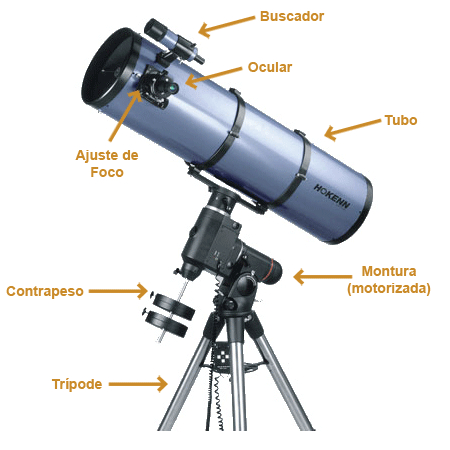
\includegraphics[width=0.5\textwidth]{./imagenes/telescopio}
\caption{Telescopio Astronómico (http://blog.astroaficion.com/)} \label{fig:telescopio}
\end{figure}

El telescopio es un instrumento cuya función principal es recoger la luz de un objeto lejano y ampliarlo. Está considerado como el artífice de la astronomía moderna.

Históricamente se le atribuye el descubrimiento a Hans Lippershey que era un fabricante de lentes, alemán, que también era científico, astrónomo e inventor.
Cuando Galileo Galilei escuchó la noticia de la creación del telescopio, decidió diseñar y construir uno, y en 1609 lo registró como el primer telescopio astronómico. Gracias a él, se pudo llevar a a cabo la destacada observación del día 7 de enero de 1610 donde se pudieron observar la existencia de cuatro de las lunas de Júpiter girando entorno al planeta.
En un principio el nombre que se le puso al instrumento fue de “lente espía”, y el 14 de abril de 1611 Giavanni Demisiani propuso el nombre de telescopio durante una cena que se brindó en honor a Galileo. Galileo decidió llevar a esa cena el telescopio y los comensales pudieron observar las lunas de Júpiter. El nombre por el que se conoce este instrumento, Telescopio, proviene del griego con el prefijo tele que significa “lejos” y se le añade la raíz griega skop que significa “ver”.

Además de poder ampliar los objetos lejanos para verlos con mayor detalle, gracias al telescopio se pueden observar cuerpos celestes de débil luminosidad y que son invisibles a simple vista, ya que el objetivo del telescopio es capaz de percibir más luz que el ojo humano. Cuanto mayor es el diámetro del objetivo, más luz capta. Dicho diámetro suele referenciarse como la “apertura del telescopio” y de ello depende el poder que tenga de resolución el objetivo y por tanto el telescopio.

Los primeros telescopios que se consolidaron fueron los de tipo kepleriano que disponían de unas longitudes focales de hasta 30 o 40 centímetros, con el objetivo de conseguir grandes aumentos.
A principios del siglo XVIII comenzaron a fabricarse los telescopios con lente y un espejo cóncavo a su vez. A partir de ese momento comenzó un debate sobre los telescopios, su utilidad y cual de ellos ofrecía mayor precisión, ya que existían dos tipos, los telescopios reflectores, en los que la luz es reflejada y dirigida hacia el foco, y los telescopios refractores, en donde  la luz es refractada pasando por el objetivo.
A mediados del siglo XX se terminó la disputa cuando triunfaron de manera definitiva los telescopios reflectores.

\subsection{Cámara CCD}
\begin{figure}[htb]
\centering
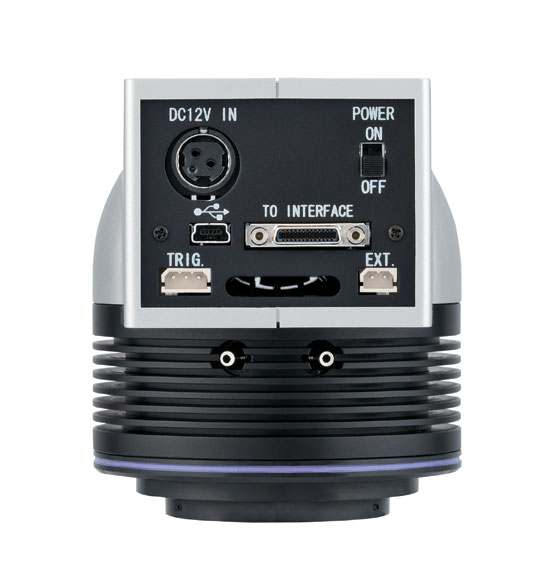
\includegraphics[width=0.4\textwidth]{./imagenes/ccd}
\caption{Cámara CCD (http://bitran.co.jp/)} \label{fig:ccd}
\end{figure}
Las siglas de cámara CCD (\textit{Charge-Coupled Device}) proceden del inglés y significan dispositivo de carga acoplada. Los primeros dispositivos que se crearon fueron inventados por Willard Boyle y George E. Smith, el 17 de octubre de 1969 dentro de los laboratorios Bell y ambos fueron distinguidos recientemente con el Premio Nobel de Física, en el año 2009, gracias a los dispositivos CCD.

Dicha cámara funciona como un detector de estado sólido. Este funcionamiento hace que la cámara sea muy eficiente ya que hace mucho más fácil la obtención y el procesamiento de las imágenes astronómicas.
La cámara CCD funciona como un conjunto de circuitos eléctricos  de condensadores enlazados y acoplados que son sensibles a la radiación electromagnética. Estos condensadores pueden transferir su carga eléctrica a uno o varios condensadores que se encuentren a su lado en el circuito impreso. El CCD registra la ubicación de cada fotodiodo sobre el que incide un fotón de rayos X. Un fotón es un paquete que contiene radiación electromagnética. A su vez, el CCD es capaz de registrar la energía que depende de su frecuencia, y por tanto, de su longitud de onda.

Los sensores CCD tienen una estructura de células que son sensibles a la luz en forma de mosaico y a cada una de esas células se le llama \textit{píxel}. Cada \textit{píxel} es una estructura detectora en la cual se pueden almacenar fotones. Desde el CCD la imagen es procesada por la cámara y a su vez registrada en la tarjeta de memoria.


\subsection{Montura}
\begin{figure}[htb]
\centering
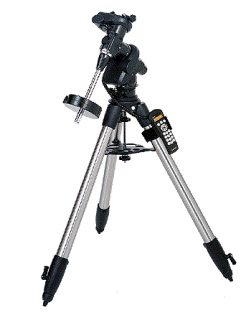
\includegraphics[width=0.5\textwidth]{./imagenes/montura}
\caption{Montura (http://astrofacil.com/)} \label{fig:montura}
\end{figure}
La montura es la parte mecánica. Sirve como estructura para montar y sujetar el tubo del telescopio y así poder realizar la operación de enfoque para poder detectar y seguir a un cuerpo celeste. Se requiere que la montura sea de mucha firmeza y a su vez tenga mucha suavidad en los movimientos para poder conseguir que las observaciones sean perfectas.

Existen varios tipos de monturas entre las que destacan: Altacimutales y Ecuatoriales.

La montura altacimutal es aquella que hace referencia al sistema de coordenadas celestes altacimutales. Requiere un continuo ajuste ya que tienen absoluta libertad para moverse en altura (de arriba hacia abajo) y en acimut (de derecha a izquierda).

La montura ecuatorial es aquella que hace referencia al sistema de coordenadas celestes ecuatoriales. Tiene un eje ecuatorial que está alineado con el eje terráqueo y algunas de estas monturas pueden disponer de un pequeño motor capaz de realizar un giro completo en 24 horas. Dispone además de otro eje, llamado declinación y es regular al primero.
Cuando se encuentra enfocado un astro y el motor se ha accionado, el tubo del telescopio sigue automáticamente el movimiento de la bóveda celeste y el objeto enfocado permanecerá fijo en el interior del campo visual del telescopio. Por este motivo tan importante, la montura ecuatorial es muy eficaz en la astronomía ya que permite exposiciones muy prolongadas.


\subsection{Enfocador}
\begin{figure}[htb]
\centering
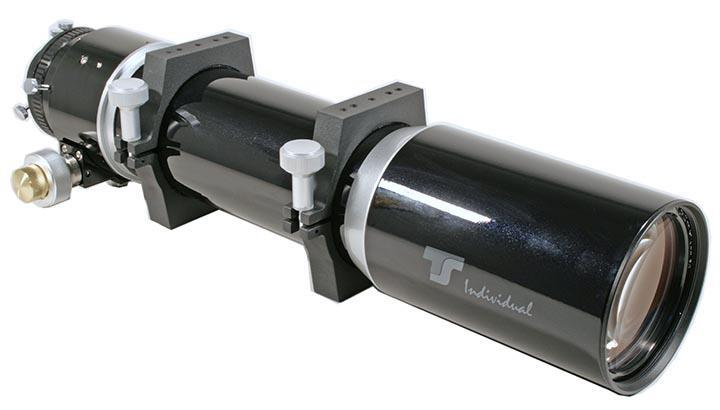
\includegraphics[width=0.5\textwidth]{./imagenes/enfocador}
\caption{Enfocador (http://tienda.lunatico.es/)} \label{fig:enfocador}
\end{figure}
El enfocador es una de las piezas fundamentales del telescopio ya que gracias a él, nos permitirá ver las imágenes formadas tras la reflexión de la luz en el espejo primario y su desviación por el espejo secundario.

Para ver las imágenes se necesitará un juego de oculares. La combinación de la longitud focal de los oculares y la longitud focal del telescopio, nos dará como resultado el número de aumentos total que tenemos en nuestro sistema.

Uno de los enfocadores más populares que existe actualmente en el mercado es el de tipo \textit{Crayford}. Estos enfocadores son bastante caros ya que tienen una relación de velocidad alta que mejora el ajuste de enfoque.


\subsection{Rueda Portafiltros}
\begin{figure}[htb]
\centering
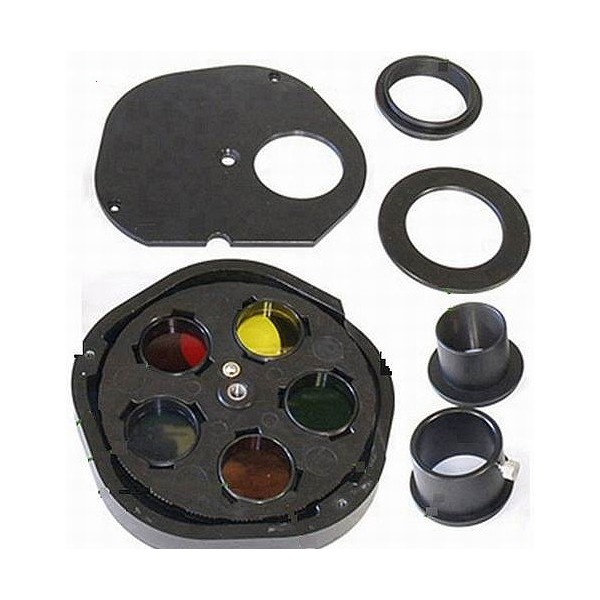
\includegraphics[width=0.5\textwidth]{./imagenes/ruedaPortafiltros}
\caption{Rueda Portafiltros (http://astrocity.es/)} \label{fig:ruedaPortafiltros}
\end{figure}
La rueda portafiltros es un objeto, generalmente de aluminio, que contiene en su interior filtros diferentes para poder cambiar de forma eficaz la visual o la astrofotografía. No hace falta quitar la cámara para cambiar el filtro ya que tan solo con un pequeño giro en la rueda se selecciona el filtro poniéndose en el lugar correcto y se puede seguir observando.
Como mínimo, se requiere que tenga cuatro filtros si se quiere realizar astrofotografía con cámaras CCD blanco y negro. Para ello, se necesitarán el filtro azul, el filtro rojo y el filtro verde (RGB), y posiblemente un filtro para los infrarrojos.


\subsection{Cúpula}
\begin{figure}[htb]
\centering
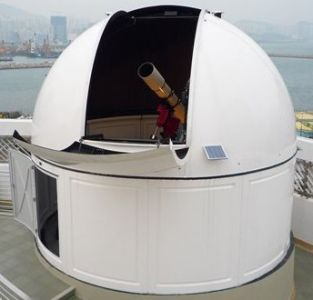
\includegraphics[width=0.4\textwidth]{./imagenes/cupula}
\caption{Cúpula Astronómica (http://apt.com.es/)} \label{fig:cupula}
\end{figure}
Una cúpula es una estructura principalmente semiesférica o de techo deslizante. La cúpula permite alojar en su interior el instrumental astronómico y protegerlo. Ya sea de un tipo o de otro, está formada por una o más escotillas que permiten su abertura y, de esta forma, poder realizar una observación.


\subsection{Óptica Adaptativa}
\begin{figure}[htb]
\centering
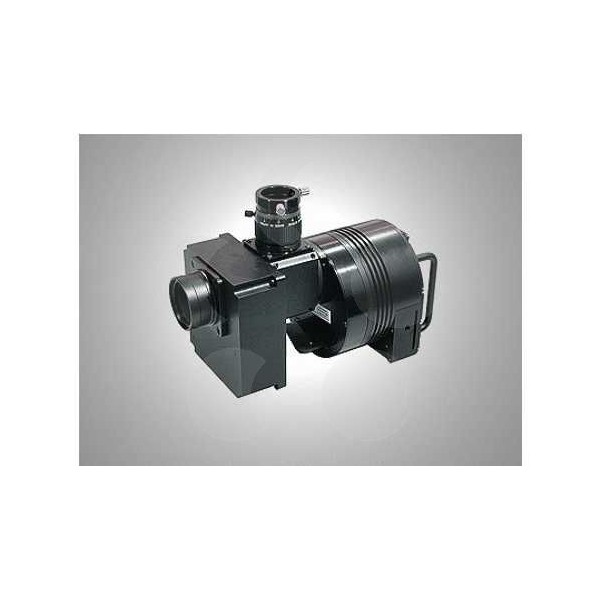
\includegraphics[width=0.3\textwidth]{./imagenes/opticaAdaptativa}
\caption{Óptica Adaptativa (http://www.valkanik.com/)} \label{fig:opticaAdaptativa}
\end{figure}
La óptica adaptativa es una técnica que permite, mediante el uso de óptica deformable, corregir en tiempo real los defectos que vienen de la atmósfera terrestre en la imagen observada con el telescopio. Es una técnica muy importante para todos los astrónomos ya que se pueden obtener imágenes mucho más nítidas. Un símil que hacen muchos astrónomos para entender esto es que la técnica es comparable con mirar un objeto situado en el fondo de una piscina con agua y sin agua.
La óptica adaptativa es capaz de eliminar las perturbaciones y por tanto equivaldría a observar desde el espacio. Ganar nitidez con la óptica en las imágenes significa concentrar en un menor número de puntos sensibles del detector los pocos fotones que llegan de los objetos débiles o lejanos y eso es, dicho con otras palabras, que la posibilidad de verlos es mayor.


\subsection{Estación Meteorológica}
\begin{figure}[htb]
\centering
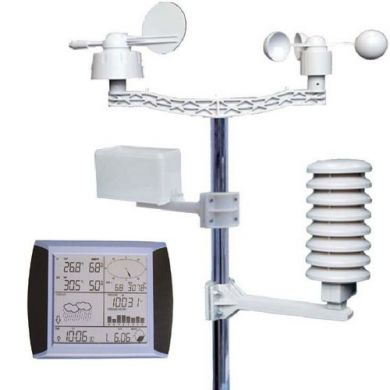
\includegraphics[width=0.4\textwidth]{./imagenes/estacionMeteorologica}
\caption{Estación Meteorológica (http://comprawifi.com/)} \label{fig:estacionMeteorologica}
\end{figure}
Una estación meteorológica es una instalación cuya función principal es medir y registrar diversos datos meteorológicos. Dichos datos se utilizan para elaborar predicciones meteorológicas a partir de modelos numéricos.
A su vez, la estación está formada por sensores e instrumentos que sirven para la obtención de todos los datos entre los que destacan el termómetro, el barómetro, el pluviómetro, el psicómetro o la veleta.


\subsection{Controlador de Dispositivos}
Hoy en día, en los observatorios, se pueden controlar los diversos instrumentos de un observatorio de diferentes formas como pueden ser:

  \begin{itemize}
    \item Controlados directamente desde el propio dispositivos.
    \item Mediante el uso de un PC y desde ahí se controlarían todos los aspectos.
    \item Mediante el uso de herramientas de control remoto. En este caso situarían al astrónomo en un lugar fuera del observatorio y desde ese lugar se podrían controlar los diferentes dispositivos que permitan realizar el trabajo del astrónomo.
  \end{itemize}


\section{Plataformas para la creación de \textit{software} astronómico}
Actualmente existen dos grandes protocolos para la creación de \textit{software} astronómico. Estos dos claros protocolos son ASCOM e INDI.  La función de ambos protocolos es llegar a poder controlar  todo el instrumental astronómico desde una misma máquina.

\section{ASCOM}
El protocolo ASCOM está formado por un conjunto de desarrolladores y fabricantes de instrumentales astronómicos. Lo que buscan lograr es la compatibilidad plug-and-play, independientemente del lenguaje que se utilice entre el \textit{software} y los instrumentos astronómicos. Para ello, crean una capa para separar los dispositivos del \textit{software} que utilizan los dispositivos. Otro objetivo es conseguir hacer que cualquier driver pueda ser utilizado en cualquier lenguaje de programación.

Tiene un gran inconveniente y es que actualmente solo funciona en sistemas operativos de \textit{Microsoft Windows} y dificulta su desarrollo ya que solamente está abierto a un único sistema operativo.

Por otra parte, hay que detallar que ASCOM no está pensado para funcionar remotamente pues su función está pensada para hacer escritorio remoto desde un sistema operativo de \textit{Microsoft Windows}.\cite{ASCOM}


!!!!!!!!!!!!!!!!!!!!IMPORTANTE!!!!!!!!!!!!!!!!!!!!
(PONER REFERENCIA A LA WEB DE ASCOM PARA ENGANCHAR CON LA BIBLIOGRAFIA)  (http://www.ascom-standards.org/)

\section{INDI}
INDI es un protocolo de \textit{software} libre diseñado para apoyar el control, la automatización, la adquisición de datos y el intercambio entre los dispositivos \textit{hardware} y las interfaces \textit{software}. Se puede usar tanto en dispositivos reales como en dispositivos virtuales.

Su biblioteca permite controlar cualquier dispositivo con un driver INDI mediante el paso de archivos del tipo XML.

INDI significa “\textit{Instrument-Neutral-Distributed-Interface}”. INDI fue creado por \textit{Elwood C. Downey} del \textit{ClearSky Institute}.

\subsection{Cómo funciona INDI}
Hoy en día, los sistemas de control que se desarrollan se hacen para una gama de dispositivos concretos o incluso para un dispositivo específico. Si se modifica algún parámetro del dispositivo o de la gama de dispositivos, el \textit{software} debe modificarse para asentar dicho cambio. En otras palabras, hay una fuerte conexión entre el \textit{software} y el \textit{backend} del \textit{hardware}.

Para que no exista esa fuerte conexión entre el \textit{software} y el \textit{backend} del \textit{hardware} se desarrolla INDI,  ya que los clientes son totalmente conscientes de las capacidades de los diferentes dispositivos que tienen conectados a través del protocolo INDI. Esto hace que en tiempo de ejecución, se construya una interfaz gráfica en función a las características que envíe el dispositivo. Dicha interfaz por tanto, se construye de forma dinámica.

\begin{figure}[htb]
\centering
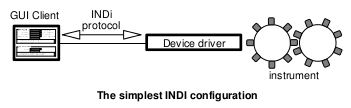
\includegraphics[width=0.6\textwidth]{./imagenes/funcionINDI}
\caption{Configuración de INDI (http://indilib.org/)} \label{fig:funcionINDI}
\end{figure}

Para que INDI funcione con total perfección se definen tres sustantivos muy importantes que hacen que encajen todas las piezas correctamente. Estos sustantivos son: \textit{drivers}, servidor y cliente.

\subsection{\textit{Drivers}, Servidores y Clientes de INDI}
\begin{itemize}
  \item El \textit{driver} de INDI es un controlador que se comunica directamente con el dispositivo. Permite conectarse a uno o más dispositivos físicos y es el responsable de definir todos los clientes. Los \textit{drivers} envían una lista de propiedades a los clientes para que éstos puedan así definir dinámicamente sus interfaces gráficas.
  \item El servidor es un programa que ejecuta los diferentes \textit{drivers} de los distintos dispositivos. Hace de conexión entre los dispositivos y los clientes. Por regla general está alojado en un ordenador en el cual están todos los dispositivos conectados. También el servidor permite que estén los dispositivos conectados en otras máquinas y éstas envíen los datos al servidor.
 Todo el intercambio de datos que se realiza entre el servidor y los \textit{drivers} se consigue mediante el uso del protocolo INDI.
  \item El cliente es un programa que hace dinámicamente la interfaz gráfica. Puede estar conectado con uno o más servidores. Una vez que conecta con uno o más servidores el cliente solicita toda la información y el servidor se la da. Seguidamente, el cliente procesa los datos y los muestra creando la interfaz que se menciona anteriormente.
\end{itemize}

\subsection{Descripción del protocolo}
El protocolo INDI define un conjunto de 5 propiedades que son las que envían los diferentes \textit{drivers} para formar la interfaz del cliente. Estas propiedades están muy relacionadas ya que una o todas las propiedades pueden estar presentes en un dispositivo. A continuación se pasa a detallar cada una de las propiedades:
\begin{itemize}
  \item \textbf{Textos:} Son cadenas de caracteres ordenados arbitrariamente.
  \item \textbf{Números:} Son cantidades numéricas. Además de la cantidad numérica se envían otros parámetros que sirven para el formato de su visualización y configuración.
  \item \textbf{Switchs:} Son propiedades que están encendidas o apagadas. Estas propiedades pueden ser de tres tipos diferentes:
    \begin{itemize}
      \item \textbf{Una de muchas:} de todas las opciones se tiene que seleccionar obligatoriamente una.
	    \item \textbf{Como máximo una:} de todas las opciones se puede seleccionar como máximo una.
	    \item \textbf{Cualquiera de muchas:} se podrán seleccionar todas las que se deseen.
    \end{itemize}
  \item \textbf{Lights:} Son propiedades que pueden estar en cada uno de los cuatro estados que se definen:
    \begin{itemize}
      \item \textbf{Inactivo:} Luz de color gris.
      \item \textbf{Alerta:} Luz de color rojo.
      \item\textbf{Ocupado:} Luz de color amarillo.
      \item \textbf{Ok:} Luz de color verde.
    \end{itemize}
  \item \textbf{Blob:} Son propiedades que tienen objetos binarios arbitrariamente, como imágenes.
\end{itemize}

\subsection{Simuladores}
INDI dispone de un conjunto de simuladores que sirven para testear todo lo que se va haciendo sin necesidad de tener un dispositivo físico. Con él se pueden realizar todo tipo de operaciones sin variar nada con respecto al dispositivo real. Entre ellos destacan:
\begin{itemize}
  \item Simulador de telescopio.
  \item Simulador de CCD.
  \item Simulador de rueda portafiltros.
  \item Simulador de enfocador.
  \item Simulador de GPS.
\end{itemize}

\section{Estado del arte. \textit{Software} con INDI y sin él}
Actualmente existen diferentes \textit{softwares} para realizar la función control de un observatorio. Hay que destacar que podemos diferenciarlos en dos grandes grupos: Los \textit{softwares} que no hacen uso de la biblioteca INDI y los que si hacen uso de dicha biblioteca.

\subsection{Clientes que no hacen uso de INDI}
\begin{itemize}
  \item \textbf{Maxim DL:} Dispone de una completa integración del observatorio y controla todo el equipo astronómico. Es compatible con ASCOM y el astrónomo puede crear sus propios preajustes. A su vez, se puede supervisar y controlar el observatorio mediante una webcam en la cúpula, interruptores remotos y vigilancia del clima. Es uno de los software sin INDI más completo que existe.
  \item \textbf{Images Plus:} Es un \textit{software} que en un principio sirve para realizar el tratamiento de astrofotografía pero que después se ha ido mejorando y hoy en día permite hacer uso y control de dispositivos. Su uso es muy limitado ya que solamente permite hacer uso de algunos dispositivos concretos. También funciona con ASCOM.
  \item \textbf{Astroplanner:} Permite planificar y ejecutar una sesión de observación al astrónomo. Se pueden introducir los sitios que se desean observar, importarlos desde archivos o buscar en el catálogo del que dispone el programa. Se puede usar tanto en MAC OS X (10.4 o superior) y en \textit{Windows} (XP o superior). Funciona también con ASCOM en la versión para \textit{Windows} pero solamente para el control de telescopios.
\end{itemize}
Referencias de los tres puntos anteriores(respectivamente):
(http://www.cyanogen.com/maximmain.php)
(http://www.mlunsold.com/ILControl.html)
(http://www.astroplanner.net/requirements.html)

\subsection{Clientes que hacen uso de INDI}
\begin{itemize}
  \item \textbf{KStars:} Es una herramienta de \textit{Software Libre} de astrofotografía incluida en multiplataforma. Proporciona una simulación gráfica precisa del cielo nocturno desde cualquier punto de la tierra. Además, proporciona herramientas de cálculo astronómico y mucha información que ayudará y facilitará el trabajo  al astrónomo.
  \item \textbf{Ekos:} Software que lleva a cabo tareas de astrofotografía bajo la plataforma Linux. Ekos es también una herramienta de \textit{Software Libre} y forma parte del \textit{software} de Kstars mencionado anteriormente.
  \item \textbf{\textit{Remote Observatory}:} Es un cliente INDI multilenguaje de \textit{Software Libre} para la plataforma Android. Se encuentra en un continuo desarrollo y permite controlar cualquier número de servidores así como múltiples interfaces.
\end{itemize}
Referencias de los tres puntos anteriores(son la misma):
http://www.indilib.org/about/clients.html

Como conclusión final diremos, que vistos algunos de los clientes que se pueden usar para llevar a cabo el control de un observatorio hay que resaltar que ninguno de ellos es capaz de llevar dicho control desde el navegador, y por tanto, necesitaríamos de un pc con unos requerimientos mínimos puesto que todos los pcs que existen en la actualidad los superarían, y una instalación del \textit{software} que, en nuestro caso, seleccionásemos.
